%%%%% START PREAMBLE HEADER %%%%%

%%% START REQUIRED PACKAGES %%%

\documentclass{article}
\usepackage[a4paper, total={7.25in, 9.5in}]{geometry} 
\usepackage{multirow}
\usepackage{lipsum}
\usepackage{hyperref}
\usepackage{listings}
\usepackage{graphicx}
\usepackage[table,xcdraw]{xcolor}
\usepackage[export]{adjustbox}
%\usepackage[superscript,biblabel]{cite}
\usepackage{amsmath}
\hypersetup{colorlinks=true,linkcolor=blue,filecolor=magenta,urlcolor=cyan,citecolor=blue}


%%% END REQUIRED PACKAGES %%%                


%%% START NEW COMMANDS new (shortcut) %%%

% This is a paragraph with normal font
\newcommand{\np}[1]{\paragraph*{\normalfont{#1}}}
% This is a text with a color
\newcommand{\ct}[2]{\textcolor{#1}{#2}}
% This is a bold text 
\newcommand{\bt}[1]{\textbf{#1}}
% This is an italic text 
\newcommand{\et}[1]{\emph{#1}}
% This is an underline text 
\newcommand{\ut}[1]{\underline{#1}}
% This is a newline shortcut
\newcommand{\n}{\\}
% This is a numbered equation with break line shortcut
\newcommand{\necbreak}[1]{\begin{equation}\begin{aligned}#1\end{aligned}\end{equation}}
% This is a numbered equation with break line shortcut
\newcommand{\nec}[1]{\begin{equation}#1\end{equation}}
% This is an equation shortcut
\newcommand{\ec}[1]{\begin{center} $#1$ \end{center}}
% Table title with bold text and correct space%
\newcommand{\titleTable}[2]{\np{\bt{Table #1} #2}}% Graph title with bold text and correct space%
\newcommand{\titleGraph}[2]{\np{\bt{Graph #1} #2}}
% Table body with border %
\newcommand{\bodyTable}[2]{\begin{center} \begin{tabular}{|#1|} \hline #2 \hline \end{tabular} \end{center} }
%%% END NEW COMMANDS (shortcuts) %%%


%%% START TITLE SETTINGS %%%
\title{\bt{2° Examen parcial Fisicoquímica de Sistemas Moleculares Organizados}}
\author{Pérez Alvarado Luis Raymundo, Facultad de Química, UNAM}
\date{~}
%%% END TITLE SETTINGS %%%

%%%%% END PREAMBLE HEADER %%%%%

%%%%%%%%%%%%%%%% START DOCUMENT %%%%%%%%%%%%%%%%
\begin{document}

    \maketitle

    % Pregunta 1 %
    \np{1) Se tienen dos proteínas (FSMO-1 y FSMO-2) cuyos parámetros termodinámicos han sido determinados experimentalmente.}

    \np{Para la proteína FSMO-1:}

    \begin{itemize}
        \item $\Delta_{unf}H(T_m)$: 390 kJ/mol
        \item $\Delta_{unf}C_p$: 3 kJ/molK
        \item $T_m$: 330 K
    \end{itemize}

    \np{Para la proteína FSMO-2:}

    \begin{itemize}
        \item $\Delta_{unf}H(T_m)$: 250 kJ/mol
        \item $\Delta_{unf}C_p$: 6 kJ/molK
        \item $T_m$: 340 K
    \end{itemize}

    \np{a) La curva de estabilidad termodinámica para cada proteína y discuta con detalle las conclusiones referentes a la estabilidad de las mismas.}

    \np{En la curva de establidad de FSMO-1 se señalan dos valores de temperatura de fusión (en estos valores la energía libre del Gibbs del proceso es cero), la que es producida por calor que proporcionó y por frio que tiene un valor de 130.2K la cual se obtuvo con la intersección de la curva que es la de enfriamiento con el eje X, con estas podemos definir el intervalo de temperatura en la que la proteína existe de forma nativa arriba de un 50\% y donde en el valor de 220K encuentra un máximo, es decir que esta completamente en su forma nativa, esto nos dice termodinamicamente que en el intervalo 150-330K de la poteína FSMO-1 es donde conformación nativa es mas estable, ya que el valor de $\Delta G_{unf}$ es positivo lo que nos indica que el proceso de desplegamiento no es favorable por lo que predomina la forma nativa, en el caso de la proteína FSMO-2 su intervalo va de 263.2-340K.}

    \np{Tambien se señalan los valores de $T_H$ y $T_S$ que son las temperaturas en los cuales los valores de $\Delta H$ y $\Delta S$ son igual a cero y se observa que se repite el mismo comportamiento en función de la temperatura y es que la pendiente arriba de dichas temperaturas es positiva y debajo de estas es negativa, esto nos muestra como varian las contribuciones entalpicas y entropicas del proceso, en el caso de FSMO-1 estas tiene valores de $T_H=200K$ y $T_S=222.6$ y el caso de FSMO-2 $T_H=298.3$ y $T_S=300.7$, esto nos sugiere que proteína FSMO-1 tiene un comportamiento parecido a un soluto no polar ya que el intervalor que hay entre $T_H$ y $T_S$ es grande}

    \np{En las gráficas de fracción mol podemos observar el domino del estado nativo en las proteína en estado nativo cuando entra al intervalo determinado por las temperaturas de fusión, donde en dicho valor de temperatura el 50\% de la proteína en estado nativo y con un pequeño cambio temperatura el 100\% de la proteía cambia de un estado a otro, dicho comportamiento se aprecia en ambas proteínas.}

    \np{b) Para cada proteína construya un segundo gráfico en donde además de estar graficado el $\Delta_{unf}G$ incluya
    $\Delta_{unf}H$ y $T\Delta_{unf}S$. En base a ese gráfico determine los valores de $T_H$ y $T_S$. Comente sus observaciones sobre las contribuciones entálpicas y entrópicas a la estabilidad de la proteína.}

    \np{c) Construya para cada proteína su gráfico de predominio de especies y su dependencia con temperatura.}

    \np{2) La constante de equilibrio, Keq, para la reacción de formación de un complejo MX,se obtuvo experimentalmente a varias temperaturas, desde 290 hasta 315 K. Los datos experimentales están registrados en la siguiente tabla.}

    \ec{M+X \rightleftharpoons MX}

    \begin{center}
        \begin{tabular}{ |c|c| } 
            \hline
             $T(K)$ & $K_{eq} (M^{-1})$  \\ 
            \hline 
            290 & $1.2x10^5$  \\ 
            \hline 
            295 & $1.3x10^5$  \\ 
            \hline
            300 & $1.4x10^5$  \\ 
            \hline
            305 & $1.5x10^5$  \\ 
            \hline
            310 & $1.6x10^5$  \\ 
            \hline
            315 & $1.7x10^5$  \\ 
            \hline 
        \end{tabular}
    \end{center}

    \np{Construya un gráfico de van’t Hoff y determine $\Delta H$, $\Delta S$ y $\Delta G$ para esta reacción a 298 K. De estos parámetros termodinámicos ¿Cuál(es) requiere(n) que se especifíque la temperatura para poder evaluarlo?}

    \np{Se realizo un gráfico de Van´t Hoff y se determinaron los valores de $\Delta H_{vh}=10.571.78 kJ/mol$ y $\Delta S_{vh}=0.13373 kJ/molT$ estos valores son constantes ya que se esta trabajando en un intervalo de temperatura pequeño en el cual no hay dependecias grandes con la temperatura.}

    \np{La energía libre depende de la temperatura, esta fue calculada a 298K usando los valores obtenidos de $\Delta H_{vh}$ y $\Delta S_{vh}$ $\Delta G_{vh}=-29.279.96 kJ/mol$}

    \np{3) En el archivo “Data.txt” se encuentra registrado la variación de la propiedad $\psi$ como función de la temperatura para el proceso de desplegamiento de la proteína XYZ, es decir el desplegamiento térmico de
    la misma. Obtenga de esta información experimental los valores de $\Delta_{unf}G$, $\Delta_{unf}H$ y $T\Delta_{unf}S$ evaluados a 298 K. Determine también la Tm de esta proteína.}

    \np{Usando las dos ecuaciones de la recta de las tendencias de cada una de los estados de la proteína observados al medir la propiedad $\psi$ la cual muestra una cambio en la propiedad al variar la temperatura y fue posible relacionar dichas ecuaciones para determinar la fracción mol con la ecuación 1 y con ello determinar el valor de $T_m=339.08K$ por medio de la gráfica de la fracción mol, esto al tomar la intersección con una recta que cruza por el 0.5 de fracción mol.}

    \nec{\Chi_U=\frac{\Theta-\Theta_N}{\Theta_U-\Theta_N}}

    \np{Por medio de considear el valor de fusión, se tomo un intervalo de 10 grados arriba y abajo para construir un grádico de Van´t Hoff para determinar sus potenciales termodinámicos se obtuvo $\Delta_{unf}G=55.872 kJ/mol$, $\Delta_{unf}H=473.099kJ/mol$ y $T_{298}\Delta_{unf}S=417.223 kJ/mol$.}


    \appendix
    % CHANGE FROM X COLUMN TO ANOTHER COLUMNS EJ 2 -> 1%
    \onecolumn
    \section{Gráficas}

    \subsection*{Pregunta 1}

    \begin{figure}[h!]
        % Reactive %
        \centering
        \begin{minipage}[b]{0.45\textwidth}
            \centering
          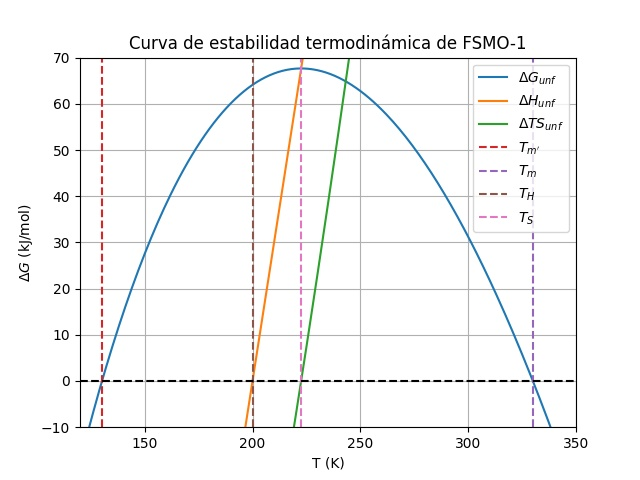
\includegraphics[scale=0.5]{g1.jpeg}
        \end{minipage}
        \begin{minipage}[b]{0.45\textwidth}
            \centering
          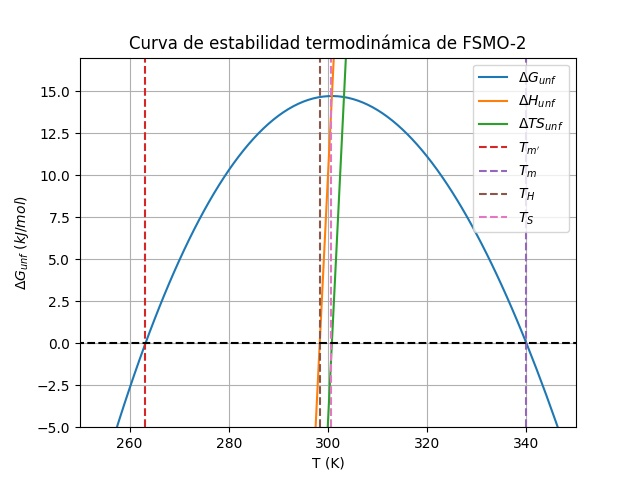
\includegraphics[scale=0.5]{fsmo21.jpeg}
        \end{minipage}
        \begin{minipage}[b]{0.45\textwidth}
            \centering
          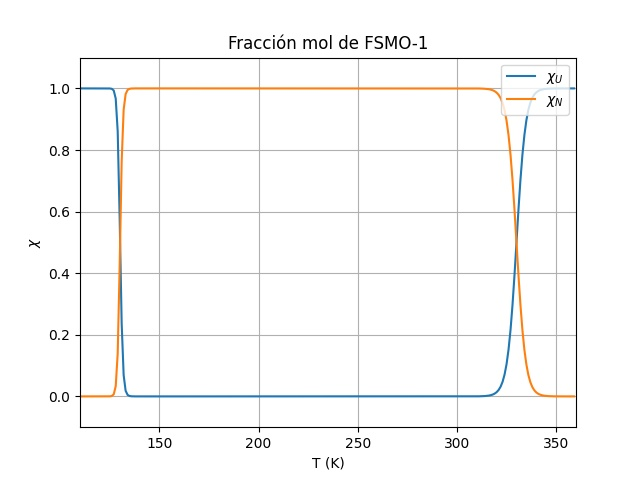
\includegraphics[scale=0.5]{fsmo12.jpeg}
        \end{minipage}
        \begin{minipage}[b]{0.45\textwidth}
            \centering
          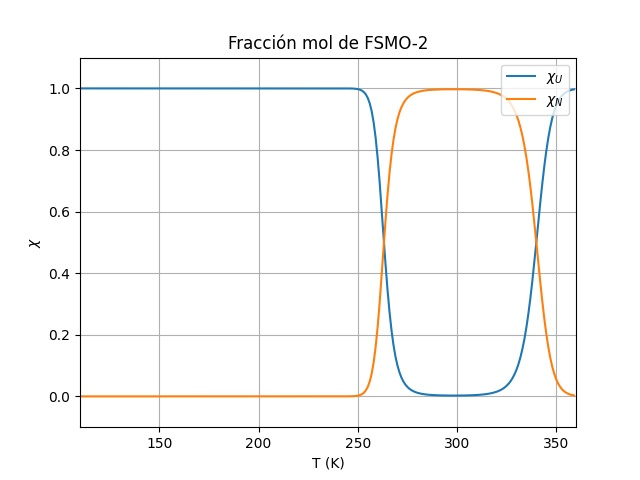
\includegraphics[scale=0.5]{fsmo22.jpeg}
        \end{minipage}
    \end{figure}
    

    \subsection*{Pregunta 2}

    \begin{center}
        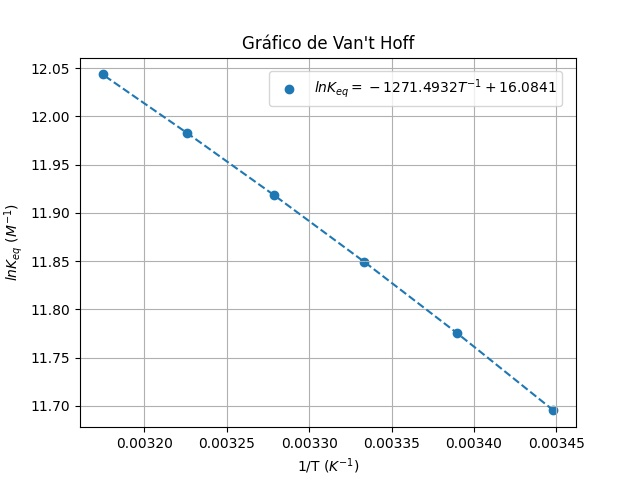
\includegraphics[scale=0.5]{g2.jpeg}
    \end{center}

    \subsection*{Pregunta 3}

    \begin{figure}[h!]
        % Reactive %
        \centering
        \begin{minipage}[b]{0.9\textwidth}
            \centering
          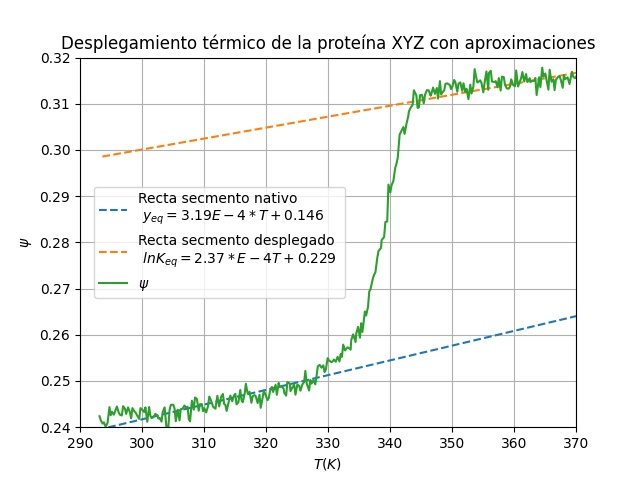
\includegraphics[scale=0.8]{g31.jpeg}
        \end{minipage}
        \begin{minipage}[b]{0.45\textwidth}
            \centering
          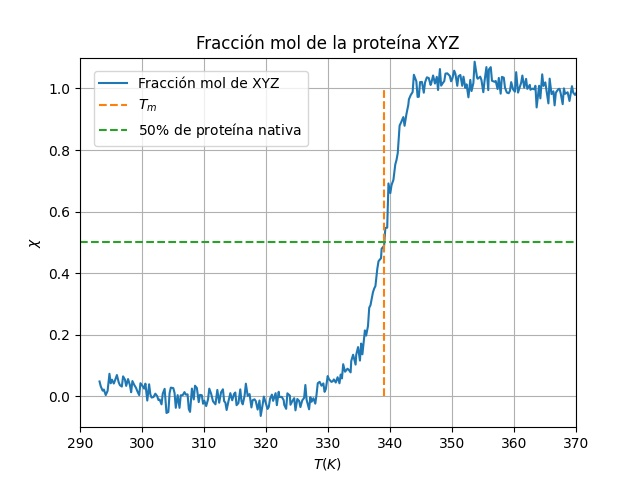
\includegraphics[scale=0.5]{g33.jpeg}
        \end{minipage}
        \begin{minipage}[b]{0.45\textwidth}
            \centering
          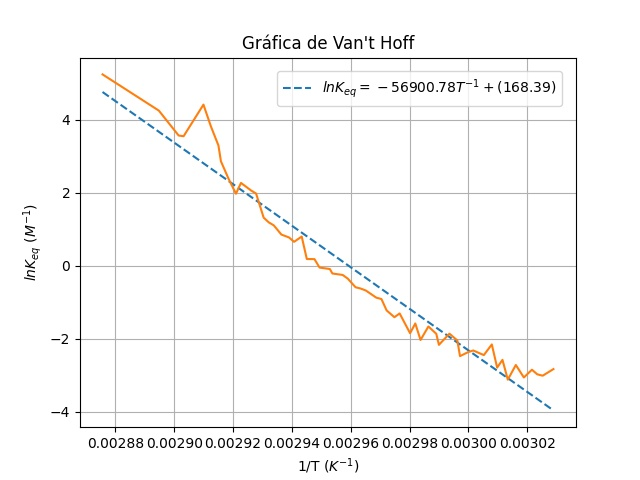
\includegraphics[scale=0.5]{g32.jpeg}
        \end{minipage}
    \end{figure}


\end{document}
%%%%%%%%%%%%%%%% END DOCUMENT %%%%%%%%%%%%%%%%